\section{Results and Discussion}

In the case of an evolutionary transition of individuality, we would expect cells to modulate their own reproductive behavior to align with group interests.
In DISHTINY, cell reproduction inherently antagonizes immediate neighbors so in the case of a transition we would expect somatic growth to occur primarily at group peripheries.
Supplementary figure \ref{fig:reproduction_surrounded} compares cellular reproduction rates between the interior and exterior of highest-level same-channel signaling networks.
In the nested treatments, this corresponded to the level-one channel and, in the flat treatments where no level-one channel was defined, this corresponded to the level-zero channel.
For all treatments, phenotypes with depressed interior cellular reproduction rates dominated across replicates (non-overlapping 95\% CI).
All four treatments appear to be sufficient to select for reproductive cooperation among cells.

Across replicate evolutionary runs in all four treatments, we also found that resource was transferred to highest-level channelmates at a significantly higher mean rate than to unrelated neighbors (non-overlapping 95\% CI).
This observation suggests that functional cooperation within same-channel groups was a common evolutionary outcome under all four treatments.
However, it could potentially be driven exclusively by resource-sharing between direct cellular kin.
We found that all four treatments exhibited mean sharing to non-direct-kin highest-level channelmates was also significantly greater than resource sharing to unrelated neighbors (non-overlapping 95\% CI).
Thus, all four treatments appear sufficient to select for functional cooperation among non-direct-kin cells.
Supplementary section \label{sec:resource-sharing} presents these results in detail.

Section \label{sec:resource-sharing} analyzes the relationship between same-channel signaling network context and cell reproduction behavior.
Then, section \ref{sec:life-histories} surveys observed multicellular life histories.

Subsequent sections describe the mechanisms and fitness effects of notable phenotypes that evolved in individual replicates.
Section \ref{sec:gene-regulation} reports a group-replication strategy mediated by gene regulation where endogenous propagule groups arise, growing to destroy the parent group.
Section \ref{sec:gradient-conditioned-behavior} describes a dynamic strategy where cells condition their own resource-sharing behavior based on a resource gradient.
Section \ref{sec:morphology} examines an example of morphological patterning of same-channel signaling networks.
Section \ref{sec:cell-cell-messaging} presents two examples of adaptive cell-cell messaging.
In the first, cell-cell messaging disrupts directional and spatial uniformity of resource sharing.
In the second, cell-cell messaging appears to intensify expression of a contextual tit-for-tat policy between same-channel signaling network groups.
Finally, section \ref{sec:apoptosis} examines replicates where widespread apoptosis evolved.

Although cooperative cell-level phenotypes were common among evolved same-channel signaling networks, across replicates functional and reproductive cooperation arose by a diverse set of qualitative life histories.

\subsection{Case Study: Burst Lifecycle} \label{sec:gene-regulation}

Across evolutionary replicates, we observed several qualitatively different life histories emerge.
Detailed in Section \ref{sec:life-histories}, these ranged from naive life histories in which parent and propagule groups exhibit no special cooperative relationship to propagules repeatedly buding off of parent groups to yield a larger network of persistent parent-child cooperators.

\begin{figure}[!htbp]
\begin{center}

\begin{subfigure}[b]{\linewidth}
\begin{center}

\begin{minipage}[t]{0.18\linewidth}
\centering
\vspace{0pt} % for alignment
\adjincludegraphics[width=\textwidth, trim={{.0\width} {.77\width} {.79\width} {.02\width}}, clip]{lifecycle/burst-paint/seed=1034+title=directional_channel_grayscale_viz+treat=resource-wave__channelsense-yes__nlev-two+update=1048648+_data_hathash_hash=ca8ad21d3b30b939+_script_fullcat_hash=602c0d0c070e9202+_source_hash=53a2252-clean+ext=}
\footnotesize Update 0
\end{minipage}
\begin{minipage}[t]{0.18\linewidth}
\centering
\vspace{0pt} % for alignment
\adjincludegraphics[width=\textwidth, trim={{.0\width} {.77\width} {.79\width} {.02\width}}, clip]{lifecycle/burst-paint/seed=1034+title=directional_channel_grayscale_viz+treat=resource-wave__channelsense-yes__nlev-two+update=1048744+_data_hathash_hash=ca8ad21d3b30b939+_script_fullcat_hash=602c0d0c070e9202+_source_hash=53a2252-clean+ext=}
\footnotesize 96
\end{minipage}
\begin{minipage}[t]{0.18\linewidth}
\centering
\vspace{0pt} % for alignment
\adjincludegraphics[width=\textwidth, trim={{.0\width} {.77\width} {.79\width} {.02\width}}, clip]{lifecycle/burst-paint/seed=1034+title=directional_channel_grayscale_viz+treat=resource-wave__channelsense-yes__nlev-two+update=1048840+_data_hathash_hash=ca8ad21d3b30b939+_script_fullcat_hash=602c0d0c070e9202+_source_hash=53a2252-clean+ext=}
\footnotesize 192
\end{minipage}
\begin{minipage}[t]{0.18\linewidth}
\centering
\vspace{0pt} % for alignment
\adjincludegraphics[width=\textwidth, trim={{.0\width} {.77\width} {.79\width} {.02\width}}, clip]{lifecycle/burst-paint/seed=1034+title=directional_channel_grayscale_viz+treat=resource-wave__channelsense-yes__nlev-two+update=1048936+_data_hathash_hash=ca8ad21d3b30b939+_script_fullcat_hash=602c0d0c070e9202+_source_hash=53a2252-clean+ext=}
\footnotesize 288
\end{minipage}
\begin{minipage}[t]{0.18\linewidth}
\centering
\vspace{0pt} % for alignment
\adjincludegraphics[width=\textwidth, trim={{.0\width} {.77\width} {.79\width} {.02\width}}, clip]{lifecycle/burst-paint/seed=1034+title=directional_channel_grayscale_viz+treat=resource-wave__channelsense-yes__nlev-two+update=1049032+_data_hathash_hash=ca8ad21d3b30b939+_script_fullcat_hash=602c0d0c070e9202+_source_hash=53a2252-clean+ext=}
\footnotesize 384
\end{minipage}
\caption{Wild type timelapse}
\label{fig:wt_timelapse}
\end{center}
\end{subfigure}

\vspace{2ex}

\begin{subfigure}[b]{\linewidth}
\begin{center}

\begin{minipage}[t]{0.30\linewidth}
\centering
\vspace{0pt} % for alignment
% adapted from https://tex.stackexchange.com/a/186476
\begin{tikzpicture}
\node[anchor=south west,inner sep=0] (image) at (0,0) { \adjincludegraphics[width=\linewidth, trim={{.25\width} {.20\width} {.5\width} {.55\width}}, clip]{knockout/interior_propagule/wildtype/seed=1+title=directional_regulator_viz+treat=resource-wave__channelsense-yes__nlev-two+update=8188+_data_hathash_hash=8b493febd79aad1f+_script_fullcat_hash=90718bb0c6ec4dbd+_source_hash=53a2252-clean+ext=}
};
\begin{scope}[x={(image.south east)},y={(image.north west)}]
  \draw [-stealth, yellow] (0.35,0.59) -- ++(0.05,-0.05);
  \draw [-stealth, yellow] (0.01,0.39) -- ++(0.05,-0.05);
  \draw [-stealth, yellow] (0.68,0.39) -- ++(0.05,-0.05);
  \draw [-stealth, yellow] (0.62,0.32) -- ++(0.05,-0.05);
\end{scope}
\end{tikzpicture}
\footnotesize Wild type
\end{minipage}
\begin{minipage}[t]{0.30\linewidth}
\centering
\vspace{0pt} % for alignment
\adjincludegraphics[width=\linewidth, trim={{.5\width} {.5\width} {.25\width} {.25\width}}, clip]{knockout/interior_propagule/propaguleknockout/seed=1+title=directional_regulator_viz+treat=resource-wave__channelsense-yes__nlev-two+update=8188+_data_hathash_hash=2b6711db47fb5887+_script_fullcat_hash=90718bb0c6ec4dbd+_source_hash=53a2252-clean+ext=}
\footnotesize Propagule knockout
\end{minipage}
\begin{minipage}[t]{0.30\linewidth}
\centering
\vspace{0pt} % for alignment
\adjincludegraphics[width=\linewidth, trim={{.5\width} {.5\width} {.25\width} {.25\width}}, clip]{knockout/interior_propagule/regulationknockout/seed=1+title=directional_regulator_viz+treat=resource-wave__channelsense-yes__nlev-two+update=8188+_data_hathash_hash=11ab5cdd47ed18c7+_script_fullcat_hash=90718bb0c6ec4dbd+_source_hash=53a2252-clean+ext=}
\footnotesize Regulation knockout
\end{minipage}

\caption{Regulation visualizations}
\label{fig:regulation_visualizations}

\end{center}
\end{subfigure}

\begin{minipage}[t]{\linewidth}
\centering
\vspace{0pt} % for alignment
\begin{subfigure}[b]{\linewidth}
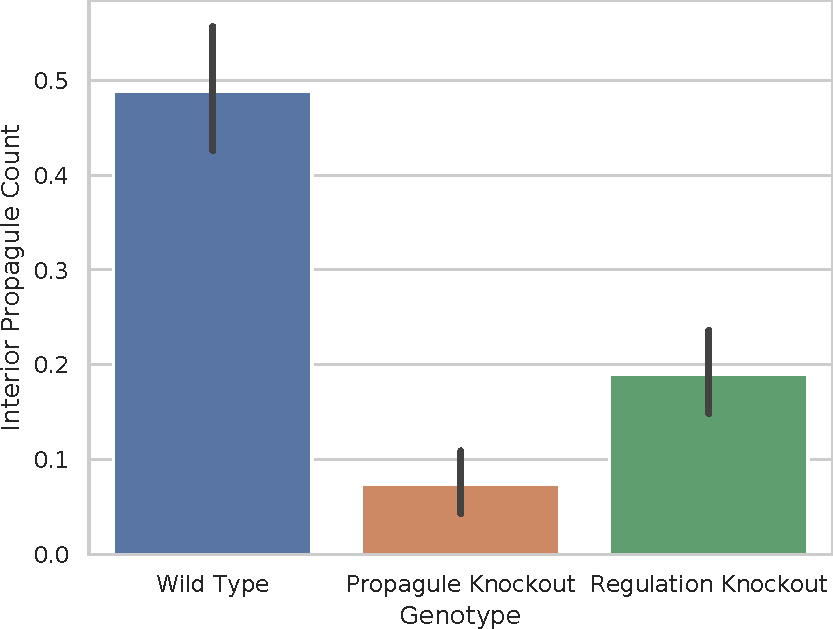
\includegraphics[width=\linewidth]{knockout/interior_propagule/title=interior_propagules+_data_hathash_hash=bb0fa6254f1b7398+_script_fullcat_hash=f738b363bea8c98a+_source_hash=53a2252-clean+ext=}%
\caption{Interior propagule rate by genotype}
\label{fig:interior_propagule_rate}
\end{subfigure}
\end{minipage}%
\hspace*{\fill}


\caption{
Analysis of a wild type strain evolved under the ``Nested-Wave'' treatment exhibiting interior propagule generation, comparing against knockouts of gene regulation and explicitly propagule-generating reproduction instructions.
Figure \ref{fig:wt_timelapse} traces the wild type life history.
Level-one groups are by differentiated by grayscale tone and separated by solid black borders.
Level-zero groups are by separated by dashed gray borders.
In each example, the focal parent level-one group is colored purple and the focal offspring group orange.
Figure \ref{fig:regulation_visualizations} depicts gene regulation at each of a cell's four directional SignalGP instances using a PCA mapping from regulatory state to three-dimensional RGB coordinates, calculated uniquely for each level-one same-channel signaling group.
Black borders divide level-one same-channel signaling groups and white borders divide level-zero same-channel signaling groups.
Endogenous daughter groups annotated with yellow arrows.
Figure \ref{fig:interior_propagule_rate} compares the mean number of interior propagules observed per level-one same-channel signaling group.
Error bars indicate 95\% confidence.
View an animation of wild type gene regulation at \url{https://mmore500.com/hopto/t}.
View the wild type strain in a live in-browser simulation at \url{https://mmore500.com/hopto/g}.
}
\label{fig:ko-interior_propagule}
\end{center}
\end{figure}


Figure \ref{fig:wt_timelapse} tracks an evolved ``burst'' life history unfolding.
In this life history, propagules arise from the interior of a parent group then replace it from the inside out.

What mechanism determines the localization and timing of the propagule origination?
This wild type strain exhibits an irregular, but somewhat concentric, spatial pattern of gene regulation illustrated in Figure \ref{fig:regulation_visualizations}.
In time-series animation, linked in the figure caption, gene regulation appears to fluctuate dynamically.

To assess mechanistic and adaptive role of gene regulation in this strain, we prepared two knockout strains.
In the first, all gene regulation instructions were replaced with Nop instructions (so that gene regulation values would remain default).
In the second, the reproduction instructions to spawn a propagule were replaced with Nop instructions.
Figure \ref{fig:regulation_visualizations} depicts the gene regulation phenotypes of these strains.

Figure \ref{fig:interior_propagule_rate} compares interior propagule generation between the strains, confirming the direct mechanistic role of gene regulation in promoting interior propagule generation (non-overlapping 95\% CI).

In head-to-head match-ups, the wild type strain outcompetes both the regulation-knockout ($20/20$; $p < 0.001$; two-tailed exact test) and the propagule-knockout strains
($20/20$; $p < 0.001$; two-tailed exact test).
The deficiency of the propagule-knockout strain confirms the adaptive role of interior propagule generation.
Likewise, the deficiency of the regulation-knockout strain affirms the adaptive role of gene regulation in the focal wild type strain.
